% ----- Fonctionnement -----

\subsection{How it works}

    To explain how our algorithm works, we will keeps track of two groups of vertices : $S$ which is a partially constructed (non-maximal) clique and the partial solution that we will gradually implement. Moreover, we also have $Z$ which is the list of all the vertices sorted according to a criteria (best degree or best sum of adjacent edge weight). Furthermore, we got $P$  which is the candidates vertices that could be included in the clique, and which represents the union of all vertex neighbors of the vertices in $S$.
    \\ \\
    The algorithm begins by forming a list of all the vertices sorted according to a criteria (best degree or best sum of adjacent edge weight). This is to facilitate the identification of the next vertices that we will add to our solution S. This makes it easier to identify the next vertices to be added to our solution S, it also saves complexity because we are not bound to check each criterion at each iteration. Then the algorithm will initialize P, and add to it all the vertices of the graph.
    \\ \\
    It will then retrieve the first element of the list Z that also belongs to P, and add it to the solution S. The selected element will then be removed from Z. After this step, $P$ is updated by considering only the neighbors of the vertices that are already part of $S$. This process is then repeated recursively until no more vertices are left in $P$, at which point the algorithm has obtained its maximum clique $S$.
    \\ \\
    To illustrate the Constructive algorithm, let's use the example in
    Figure \ref{fig:basic-graph-example} on page \pageref{fig:basic-graph-example} while adding some weight to its edges: \\

    \begin{minipage}{\linewidth}
        \textbf{Step 0:} \newline
        \begin{minipage}{0.4\textwidth}
            \begin{figure}[H]
                \centering
                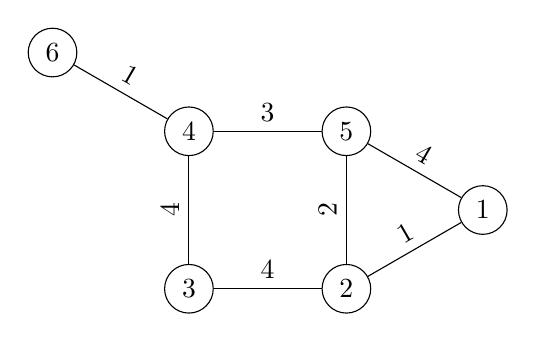
\begin{tikzpicture}[node distance=2cm]
                    \node[circle, draw] (1) {1};
                    \node[circle, draw] (2) at ([shift=(210:2)] 1) {2};
                    \node[circle, draw] (3) [left of=2] {3};
                    \node[circle, draw] (4) [above of=3] {4};
                    \node[circle, draw] (5) [above of=2] {5};
                    \node[circle, draw] (6) at ([shift=(150:2)] 4) {6};
    
                    \draw  (1) -- (2) node[midway, above, sloped] {1};
                    \draw (1) -- (5) node[midway, above, sloped] {4};
                    \draw (2) -- (3) node[midway, above, sloped] {4};
                    \draw (2) -- (5) node[midway, above, sloped] {2};
                    \draw (3) -- (4) node[midway, above, sloped] {4};
                    \draw (4) -- (5) node[midway, above, sloped] {3};
                    \draw (4) -- (6) node[midway, above, sloped] {1};
                \end{tikzpicture}
                \caption{Graph illustration for the constructive algorithm at step 0}
                \label{fig:constructive-mewc-maxedge-step0}
            \end{figure}
        \end{minipage}
        \begin{minipage}{0.6\textwidth}
            At the initial step, as said before, we will initialize $S$, $P$ and $Z$ by sorting the vertices based on a criteria. Here we chose the vertex with highest sum of weights of its edges.
            \begin{center}
                \begin{tabular}{|lll|}
                    \hline
                    S = \{$\emptyset$\} & P = \{1,2,3,4,5,6\} & Z = \{5,3,4,2,1,6\} \\
                    \hline
                \end{tabular}
            \end{center}
        \end{minipage}
    \end{minipage} 
    
    \vspace{1\baselineskip}

    \begin{minipage}{\linewidth}
        \textbf{Step 1:} \newline
        \begin{minipage}{0.4\textwidth}
            \begin{figure}[H]
                \centering
                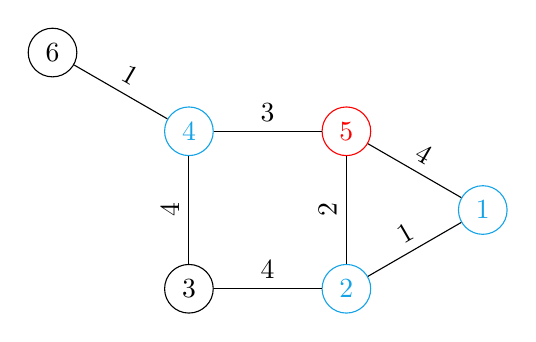
\begin{tikzpicture}[node distance=2cm]
                    \node[circle, draw, Cerulean] (1) {1};
                    \node[circle, draw, Cerulean] (2) at ([shift=(210:2)] 1) {2};
                    \node[circle, draw] (3) [left of=2] {3};
                    \node[circle, draw, Cerulean] (4) [above of=3] {4};
                    \node[circle, draw, red] (5) [above of=2] {5};
                    \node[circle, draw] (6) at ([shift=(150:2)] 4) {6};
    
                    \draw  (1) -- (2) node[midway, above, sloped] {1};
                    \draw (1) -- (5) node[midway, above, sloped] {4};
                    \draw (2) -- (3) node[midway, above, sloped] {4};
                    \draw (2) -- (5) node[midway, above, sloped] {2};
                    \draw (3) -- (4) node[midway, above, sloped] {4};
                    \draw (4) -- (5) node[midway, above, sloped] {3};
                    \draw (4) -- (6) node[midway, above, sloped] {1};
                \end{tikzpicture}
                \caption{Graph illustration for the constructive algorithm at step 1}
                \label{fig:constructive-mewc-maxedge-step1}
            \end{figure}
        \end{minipage}
        \begin{minipage}{0.6\textwidth}
            In step 1, the algorithm will take the first vertex of $Z$ if it is common to $P$ (here 5). He will then add it to $S$, represented in \textcolor{red}{red} . $P$, represented in \textcolor{Cerulean}{blue}, will be updated by taking only the vertices that are neighbors to all the members of $S$ (here, $S$ is composed only of vertex 5, so we take only the neighbors of 5).
    
            \begin{center}
                \begin{tabular}{|lll|}
                    \hline
                    S = \{5\} & P = \{4,2,1\} & Z = \{3,4,2,1,6\} \\
                    \hline
                \end{tabular}
            \end{center}
        \end{minipage}
    \end{minipage} 

    \vspace{1\baselineskip}

    \begin{minipage}{\linewidth}
        \textbf{Step 2:} \newline
        \begin{minipage}{0.4\textwidth}
            \begin{figure}[H]
                \centering
                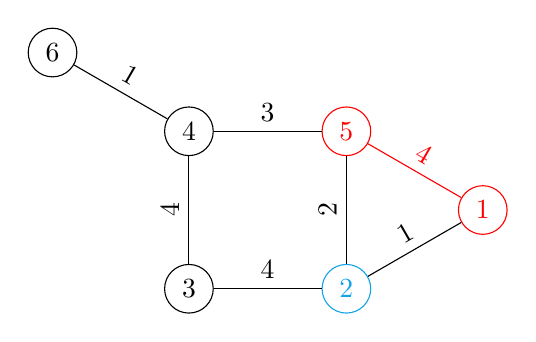
\begin{tikzpicture}[node distance=2cm]
                    \node[circle, draw, red] (1) {1};
                    \node[circle, draw, Cerulean] (2) at ([shift=(210:2)] 1) {2};
                    \node[circle, draw] (3) [left of=2] {3};
                    \node[circle, draw] (4) [above of=3] {4};
                    \node[circle, draw, red] (5) [above of=2] {5};
                    \node[circle, draw] (6) at ([shift=(150:2)] 4) {6};
    
                    \draw  (1) -- (2) node[midway, above, sloped] {1};
                    \draw[red] (1) -- (5) node[midway, above, sloped] {4};
                    \draw (2) -- (3) node[midway, above, sloped] {4};
                    \draw (2) -- (5) node[midway, above, sloped] {2};
                    \draw (3) -- (4) node[midway, above, sloped] {4};
                    \draw (4) -- (5) node[midway, above, sloped] {3};
                    \draw (4) -- (6) node[midway, above, sloped] {1};
                \end{tikzpicture}
                \caption{Graph illustration for the constructive algorithm at step 2}
                \label{fig:constructive-mewc-edge-step2}
            \end{figure}
        \end{minipage}
        \begin{minipage}{0.6\textwidth}
            In step 2, the algorithm will repeat the process of step 1 by making a recursive call until $P$ is empty. We can note in the process that our algorithm iterates again on some elements of Z, deleting them and refactoring the list does not improve the complexity, but implementing it as we did improves it in general(by not checking every neighbors each times). 
    
            \begin{center}
                \begin{tabular}{|lll|}
                    \hline
                    S = \{5,1\} & P = \{2\} & Z = {3,4,2,6} \\
                    \hline
                \end{tabular}
            \end{center}
        \end{minipage}
    \end{minipage}

    \vspace{1\baselineskip}

    \begin{minipage}{\linewidth}
        \textbf{Step 2:} \newline
        \begin{minipage}{0.4\textwidth}
            \begin{figure}[H]
                \centering
                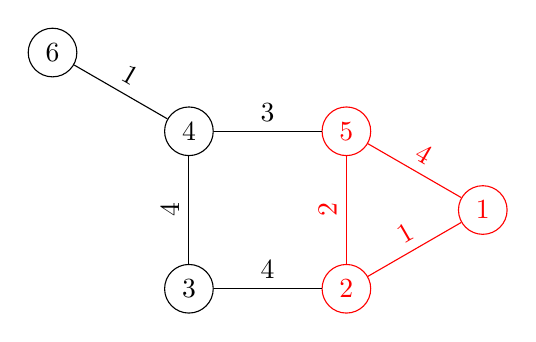
\begin{tikzpicture}[node distance=2cm]
                    \node[circle, draw, red] (1) {1};
                    \node[circle, draw, red] (2) at ([shift=(210:2)] 1) {2};
                    \node[circle, draw] (3) [left of=2] {3};
                    \node[circle, draw] (4) [above of=3] {4};
                    \node[circle, draw, red] (5) [above of=2] {5};
                    \node[circle, draw] (6) at ([shift=(150:2)] 4) {6};
    
                    \draw[red]  (1) -- (2) node[midway, above, sloped] {1};
                    \draw[red] (1) -- (5) node[midway, above, sloped] {4};
                    \draw (2) -- (3) node[midway, above, sloped] {4};
                    \draw[red] (2) -- (5) node[midway, above, sloped] {2};
                    \draw (3) -- (4) node[midway, above, sloped] {4};
                    \draw (4) -- (5) node[midway, above, sloped] {3};
                    \draw (4) -- (6) node[midway, above, sloped] {1};
                \end{tikzpicture}
                \caption{Graph illustration for the constructive algorithm at step 3}
                \label{fig:constructive-mewc-edge-step3}
            \end{figure}
        \end{minipage}
        \begin{minipage}{0.6\textwidth}
            In step 3, the algorithm repeat the step 1 by making a recursive call. It will finally find 2 which is the last vertex of $P$. The algorithm stop and we get the maximmum clique in \textcolor{red}{red} $(1,2,5)$.
    
            \begin{center}
                \begin{tabular}{|lll|}
                    \hline
                    S = \{5,1\} & P = \{2\} & Z = {3,4,2,6} \\
                    \hline
                \end{tabular}
            \end{center}
        \end{minipage}
    \end{minipage}

    \vspace{1\baselineskip}

    Now we calculate the weight of this clique. The constructive algorithm is now finished and we have obtained the following maximum clique of weight 7 : $$(1,2,5)$$

\newpage

